\documentclass{beamer}

%% Tema y configuraciones (misma anatomía de mis otros cursos)
\usetheme{Boadilla}
\usecolortheme{default}
\setbeamertemplate{navigation symbols}{}
\usepackage[utf8]{inputenc}
\usepackage{xcolor}
\usepackage{graphicx}
\usepackage{booktabs}
\usepackage{array}
\usepackage{colortbl}
\hypersetup{
    colorlinks=true,
    linkcolor=.,
    urlcolor=blue,
    citecolor=.,
}

%% Colores del semáforo y de apoyo
\definecolor{verdeok}{RGB}{39,124,74}
\definecolor{rojoal}{RGB}{198,40,40}
\definecolor{naranjal}{RGB}{230,126,34}
\definecolor{amarillal}{RGB}{240,195,60}
\definecolor{grisclaro}{RGB}{242,243,246}
\definecolor{azulcaso}{RGB}{28,60,120}

%% Encabezado
\title[06327-ECO]{Analítica para los negocios \\ 06327-ECO}
\subtitle{Semana 05: De la necesidad a la pregunta --- y de la pregunta al producto}
\author{Eduard F. Martínez González, Ph.D.}
\institute[]{Departamento de Economía, Universidad Icesi}
\date{1 de septiembre de 2026}

%%=================================================
%% Begin document
\begin{document}

%%=================================================
%% Primer slide
\begin{frame}
\titlepage
\end{frame}

%%=================================================
%% Objetivo de la sesión
\begin{frame}{Objetivo de la sesión}
\small
Hoy no abrimos RStudio: hoy practicamos \textbf{el oficio de pensar como analista}.

\vspace{0.15cm}
\begin{itemize} \setlength{\itemsep}{0.18cm}
  \item Vamos a recorrer \textbf{dos proyectos reales de consultoría} --- dirigidos desde el centro de investigación de la universidad --- desde la necesidad vaga del cliente hasta el producto final entregado.
  \item En cada paso vamos a \textbf{reconocer los conceptos del podcast}: los tres criterios de una buena pregunta, el test de la pregunta, las siete etapas y los tipos de tarea analítica.
  \item Los dos casos arrancan en puntos \textbf{opuestos}: en uno \emph{no existían los datos}; en el otro \emph{sobraban}. Esa diferencia lo cambia todo.
  \item Al final, el método queda en sus manos: \textbf{leer el caso Cóndor, entender sus datos y proponer la pregunta de negocio de su grupo} --- el insumo directo de la Entrega 1.
\end{itemize}

\vspace{0.2cm}
\begin{block}{La idea que gobierna la sesión}
Un proyecto de analítica no es exitoso porque el modelo acierte: es exitoso cuando \textbf{cambia una decisión}. Hoy lo veremos dos veces, con proyectos que sí ocurrieron.
\end{block}
\end{frame}

%%=================================================
%% Dónde estamos en el curso
\begin{frame}{¿Dónde estamos en el curso?}
\small
\begin{itemize} \setlength{\itemsep}{0.24cm}
  \item \textbf{Semanas 1--4:} las herramientas. R y los scripts reproducibles, \texttt{dplyr} para transformar, \texttt{ggplot2} para graficar. La semana pasada fuimos \emph{del dato a la gráfica}.
  \item \textbf{Semana 5 (esta):} el mapa. El proceso analítico completo: de la pregunta a la decisión. La semana 4 entera era apenas \emph{una} de las siete etapas.
  \item \textbf{Hoy en clase:} el mapa aplicado dos veces, con casos reales --- y luego ustedes lo aplican por primera vez a su proyecto.
  \item \textbf{Semana 6:} EDA y calidad de datos --- la etapa donde se va el 80\% del tiempo.
  \item \textbf{Semana 7:} examen parcial 1 (unidades 1 a 5).
\end{itemize}

\vspace{0.15cm}
\begin{alertblock}{El proyecto final arranca hoy}
La \textbf{Entrega 1} pide exactamente lo que vamos a practicar: la pregunta de negocio de su grupo sobre el caso Cóndor. Lo que salga de la clase de hoy es su materia prima.
\end{alertblock}
\end{frame}

%%=================================================
%% Tabla de contenidos
\begin{frame}[noframenumbering]{Roadmap}
\tableofcontents
\end{frame}

%%=================================================
%% SECCIÓN 1: EL MAPA
%%=================================================
\section{El mapa que ya tienen (repaso en una lámina)}

\begin{frame}[noframenumbering]{Roadmap}
\tableofcontents[currentsection]
\end{frame}

%%=================================================
\begin{frame}{Todo el podcast, en una lámina}
\footnotesize
\begin{columns}[T]
\column{0.48\textwidth}
\textbf{Una buena pregunta de negocio}
\begin{enumerate} \itemsep2pt
  \item \textbf{Específica} --- ¿qué, quién, cuándo?
  \item \textbf{Accionable} --- ¿qué decisión cambia?
  \item \textbf{Medible} --- ¿existen datos para responderla?
\end{enumerate}
\vspace{0.2cm}
\begin{block}{El test de la pregunta}
Si te doy la respuesta ahora mismo, \textbf{¿sabes qué vas a hacer diferente mañana?} Si no: tienes un tema, no una pregunta.
\end{block}
\vspace{0.2cm}
\textbf{Las siete etapas (y un ciclo)} \\
pregunta $\to$ datos $\to$ limpieza $\to$ EDA $\to$ modelo $\to$ comunica $\to$ decide $\to$ \emph{(y de vuelta)}

\column{0.48\textwidth}
\textbf{Las cinco tareas analíticas}
\begin{center}
\begin{tabular}{@{}lll@{}}
\toprule
\textbf{Tarea} & \textbf{¿Target?} & \textbf{Output} \\
\midrule
Clasificación & sí & categoría \\
Predicción & sí & número \\
Segmentación & no & grupos \\
Anomalías & mixto & lista de raros \\
Optimización & --- & decisión \\
\bottomrule
\end{tabular}
\end{center}
\vspace{0.3cm}
\begin{alertblock}{Hoy}
Dos recorridos completos por este mapa. Su trabajo: ir marcando \emph{en qué etapa estamos} y \emph{qué tarea es}.
\end{alertblock}
\end{columns}
\end{frame}

%%=================================================
%% SECCIÓN 2: CASO A
%%=================================================
\section{Caso A --- Empresa P: predecir un mercado que no está en los datos}

\begin{frame}[noframenumbering]{Roadmap}
\tableofcontents[currentsection]
\end{frame}

%%=================================================
\begin{frame}{Caso A · El contexto}
\small
\textbf{Empresa P} es una multinacional de \textbf{empaques de cartón}. Una parte importante de su negocio depende de un cliente muy concreto: \textbf{los exportadores de fruta} de América Latina --- cada tonelada de fruta que sale del continente viaja en sus cajas.

\vspace{0.3cm}
\textbf{El problema que la desvela:} el cambio climático está moviendo el mapa frutícola mundial. Zonas que hoy producen dejarán de hacerlo; otras que hoy no pesan, despegarán. Y las inversiones de la empresa (plantas, capacidad, relaciones comerciales) se deciden \emph{años antes}. \pause

\vspace{0.3cm}
\begin{exampleblock}{La necesidad, tal como llegó}
\centering \emph{``Queremos entender hacia dónde debemos orientar nuestro trabajo futuro \\ en este mercado.''}
\end{exampleblock}

\vspace{0.2cm}
\textbf{¿Qué tiene de vaga?} No dice \emph{qué} medir, ni \emph{dónde}, ni \emph{a qué horizonte}, ni \emph{qué decisión} está esperando la respuesta. Es una inquietud legítima --- pero todavía no se puede trabajar. \textbf{Convertir esto en una pregunta es la etapa 1 del proceso.}
\end{frame}

%%=================================================
\begin{frame}{Caso A · La pregunta de negocio}
\small
\begin{block}{De la necesidad vaga\ldots\ a la pregunta que dispara el proyecto}
\centering
\emph{``¿Cómo evolucionarán las \textbf{exportaciones de fruta} (toneladas), \textbf{por país y por tipo de fruta}, hacia \textbf{2045} bajo distintos \textbf{escenarios de temperatura} --- y dónde crecerá o caerá la demanda potencial de empaques?''}
\end{block}
\pause
\vspace{0.12cm}
¿Cumple los tres criterios?
\begin{itemize} \itemsep2pt
  \item \textcolor{verdeok}{\textbf{Específica}} --- qué: exportaciones en toneladas; quién: 14 países productores y competidores, fruta por fruta; cuándo: horizonte 2025--2045.
  \item \textcolor{verdeok}{\textbf{Accionable}} --- prioriza \emph{dónde} enfocar la estrategia comercial y qué mercados vigilar. Test de la pregunta: con la respuesta en la mano, mañana la agenda cambia.
  \item \textcolor{verdeok}{\textbf{Medible}} --- \emph{casi}: hay historial de exportaciones y hay escenarios climáticos\ldots\ pero \textbf{nadie los ha juntado}. Ahí está todo el proyecto. \pause
\end{itemize}

\vspace{0.12cm}
\begin{alertblock}{¿Qué tarea analítica es?}
Output = \textbf{número} (toneladas futuras) + historial con la respuesta correcta $\Rightarrow$ \textbf{predicción, supervisada}.
\end{alertblock}
\end{frame}

%%=================================================
\begin{frame}{Caso A · El problema: la respuesta no estaba en ningún dataset}
\small
No existía ninguna base de ``exportaciones frutícolas condicionadas al clima''. \textbf{Hubo que construirla} desde fuentes abiertas --- la etapa 2 fue el corazón del proyecto:

\vspace{0.25cm}
\begin{columns}[T]
\column{0.46\textwidth}
\begin{block}{\footnotesize El target (Y)}
\footnotesize Exportaciones de fruta en \textbf{toneladas}, por país--fruta--año: series históricas de \textbf{FAO}.
\end{block}
\column{0.5\textwidth}
\begin{block}{\footnotesize Las explicativas (X)}
\footnotesize Temperatura histórica y \textbf{proyectada} por país: portal climático del \textbf{Banco Mundial} (CCKP), bajo \textbf{tres escenarios} de emisiones (SSP1-1.9 optimista · SSP2-4.5 moderado · SSP5-8.5 intensivo).
\end{block}
\end{columns}

\vspace{0.25cm}
El resultado: un \textbf{panel país--fruta--tiempo} armonizado --- con rezagos, tendencias y transformaciones construidas a mano. \pause

\vspace{0.15cm}
\begin{alertblock}{La regla 80/20, en vivo}
La mayor parte del esfuerzo se fue en \textbf{encontrar, integrar y validar} datos de fuentes distintas. El modelo vino después --- y fue lo más rápido.
\end{alertblock}
\end{frame}

%%=================================================
\begin{frame}{Caso A · El análisis}
\small
\begin{enumerate} \setlength{\itemsep}{0.22cm}
  \item \textbf{Modelos supervisados} entrenados sobre el panel: Random Forest, XGBoost y una red neuronal --- tres algoritmos compitiendo por capturar la relación clima--exportaciones (que no tiene por qué ser lineal).
  \item \textbf{Validación fuera de muestra con enfoque temporal}: se entrena con el pasado y se evalúa contra años que el modelo \emph{no vio}, respetando el orden del tiempo. Métricas de error de predicción (MAE, RMSE, MAPE) por fruta y país.
  \item \textbf{Selección del mejor modelo} por desempeño y estabilidad --- no por sofisticación.
  \item \textbf{Proyección}: al modelo ganador se le inyectan las trayectorias de temperatura de cada escenario SSP, y produce las exportaciones esperadas hacia 2045.
\end{enumerate}
\pause
\vspace{0.15cm}
\begin{block}{Conecta con la teoría}
``No se evalúa un modelo con los datos con los que se entrenó'': aquí el examen de verdad es predecir años que el modelo no vio. (Volvemos a esto en la semana 10.)
\end{block}
\end{frame}

%%=================================================
\begin{frame}{Caso A · El producto final}
\small
Un \textbf{informe prospectivo ejecutivo}: resumen gerencial, escenarios, y un cuadro que prioriza las combinaciones país--fruta con mayor expansión y mayor contracción a 2045. Una muestra real (escenario moderado SSP2-4.5, variación 2045 vs.\ promedio 2020--2024):

\vspace{0.3cm}
\begin{center}
\small
\begin{tabular}{@{}llrr@{}}
\toprule
\textbf{País} & \textbf{Fruta} & \textbf{Variación a 2045} & \textbf{Particip.\ mercado 2045} \\
\midrule
\rowcolor{grisclaro} Colombia & limones & \textcolor{verdeok}{\textbf{+248\%}} & 3,5\% \\
Estados Unidos & frambuesas & \textcolor{verdeok}{\textbf{+108\%}} & 60,5\% \\
\rowcolor{grisclaro} México & aguacates & \textcolor{verdeok}{\textbf{+50\%}} & 49,2\% \\
Guatemala & melones & \textcolor{rojoal}{\textbf{--43\%}} & 20,4\% \\
\rowcolor{grisclaro} Brasil & piña & \textcolor{rojoal}{\textbf{--87\%}} & 0,1\% \\
\bottomrule
\end{tabular}
\end{center}

\vspace{0.3cm}
\pause
Miren dos filas: Colombia--limones y Brasil--piña tienen las variaciones \textbf{más espectaculares} de la tabla\ldots\ y las participaciones de mercado \textbf{más pequeñas}. ¿Entonces qué se recomienda? $\to$ \emph{siguiente lámina.}
\end{frame}

%%=================================================
\begin{frame}{Caso A · La lectura de negocio (la cuarta pata)}
\small
El modelo produce números; \textbf{el analista produce prioridades}. La clave: la \emph{doble lectura} --- variación proyectada $\times$ participación de mercado.

\vspace{0.15cm}
\begin{itemize} \setlength{\itemsep}{0.18cm}
  \item \textbf{Colombia, limones (+248\%, part.\ 3,5\%)} $\to$ \emph{oportunidad emergente}: crece muchísimo, pero desde una base pequeña. Se vigila; no redefine la estrategia.
  \item \textbf{EE.UU., frambuesas (+108\%, part.\ 60,5\%)} $\to$ \emph{foco material}: crecimiento alto \textbf{y} dominio del mercado. Aquí sí se mueve capacidad.
  \item \textbf{Guatemala, melones (--43\%, part.\ 20,4\%)} $\to$ \emph{riesgo prioritario}: cae fuerte en un mercado donde el país pesa.
  \item \textbf{Brasil, piña (--87\%, part.\ 0,1\%)} $\to$ espectacular\ldots\ e \emph{irrelevante} para la decisión.
\end{itemize}
\pause
\vspace{0.12cm}
\begin{alertblock}{El error del analista junior}
Presentar la tabla ordenada por variación y detenerse ahí. El +248\% \emph{sin} el 3,5\% al lado manda la estrategia al lugar equivocado. \textbf{Esa columna extra es el enfoque de negocio.}
\end{alertblock}
\end{frame}

%%=================================================
\begin{frame}{Caso A · Del producto a la decisión}
\small
\begin{columns}[T]
\column{0.58\textwidth}
\textbf{Lo que la empresa hizo con el informe:}
\begin{itemize} \itemsep4pt
  \item Priorizar \textbf{dónde} enfocar la estrategia comercial de los próximos años (focos de expansión con peso de mercado).
  \item Construir una \textbf{lista de vigilancia} de riesgos: mercados relevantes con contracción proyectada.
  \item Cruzar los focos con \textbf{riesgos no climáticos} (logística, concentración productiva) antes de decidir.
\end{itemize}
\vspace{0.2cm}
El entregable se lee \textbf{una vez} y alimenta decisiones de \textbf{largo plazo}. Es un producto tipo \emph{informe}.

\column{0.4\textwidth}
\begin{block}{\footnotesize Ficha del proyecto}
\footnotesize
\begin{itemize} \itemsep2pt
  \item Duración: \textbf{3 semanas}.
  \item Entrega: \textbf{única} (informe + nota metodológica).
  \item Etapas dominantes: \textbf{1--3} (pregunta y construcción de datos).
  \item Tarea: \textbf{predicción} supervisada.
  \item Roles protagonistas: \emph{business analyst} + \emph{data engineer}.
\end{itemize}
\end{block}
\end{columns}
\end{frame}

%%=================================================
%% SECCIÓN 3: CASO B
%%=================================================
\section{Caso B --- Empresa M: vigilar una red que produce datos sin parar}

\begin{frame}[noframenumbering]{Roadmap}
\tableofcontents[currentsection]
\end{frame}

%%=================================================
\begin{frame}{Caso B · El contexto}
\small
\textbf{Empresa M} es una empresa de \textbf{servicios públicos domiciliarios}: atiende $\sim$1,4 millones de usuarios residenciales y opera una red con $\sim$300 \textbf{estaciones telemedidas} que registran el consumo \textbf{hora a hora}.

\vspace{0.25cm}
\textbf{Cómo se vigila esa red hoy:} un profesional llega a las 7:00 a.m., saca el reporte del día anterior de los grandes consumidores y lo compara contra un día típico. La regla vigente obliga a revisar en detalle \textbf{toda variación mayor al $\pm$20\%}. Estación por estación. En hoja de cálculo. \pause

\vspace{0.25cm}
\begin{columns}[T]
\column{0.55\textwidth}
\begin{exampleblock}{La necesidad, tal como llegó}
\centering \emph{``Necesitamos detectar consumos atípicos a tiempo --- sin ahogarnos revisando estación por estación.''}
\end{exampleblock}
\column{0.42\textwidth}
\begin{block}{\footnotesize El número que le duele al negocio}
\footnotesize Mantener las \textbf{pérdidas} --- la diferencia entre lo medido a la entrada de la red y lo facturado a clientes --- \textbf{por debajo del 1\%}. Cada anomalía no detectada es pérdida, fraude o falla que nadie vio.
\end{block}
\end{columns}

\vspace{0.2cm}
A diferencia de la Empresa P, aquí \textbf{los datos sobran}: millones de lecturas horarias. El problema es convertirlas en \emph{decisión diaria}.
\end{frame}

%%=================================================
\begin{frame}{Caso B · La pregunta de negocio}
\small
\begin{block}{De la necesidad vaga\ldots\ a la pregunta operativa}
\centering
\emph{``¿Qué estaciones se desviaron \textbf{ayer} de su consumo \textbf{esperado} --- y en qué horas --- para priorizar la revisión de \textbf{hoy}?''}
\end{block}
\pause
\vspace{0.15cm}
\begin{itemize} \itemsep3pt
  \item \textcolor{verdeok}{\textbf{Específica}} --- qué estación, qué horas, qué día. Nada de ``consumos raros en general''.
  \item \textcolor{verdeok}{\textbf{Accionable}} --- la respuesta \emph{es} la lista de trabajo del turno de la mañana. Test de la pregunta: aprobado por diseño.
  \item \textcolor{verdeok}{\textbf{Medible}} --- un año de lecturas horarias ya almacenadas.
\end{itemize}

\vspace{0.12cm}
(El mismo proyecto tiene una \textbf{pregunta gemela} para la fase residencial: ¿qué usuarios muestran patrones atípicos compatibles con fraude? --- misma lógica, otra escala.) \pause

\vspace{0.12cm}
\begin{alertblock}{¿Qué tarea analítica es?}
``¿Qué es \textbf{raro} aquí?'' $\Rightarrow$ \textbf{detección de anomalías}. La palabra clave es \emph{esperado}: sin un \textbf{baseline}, ``anómalo'' no significa nada.
\end{alertblock}
\end{frame}

%%=================================================
\begin{frame}{Caso B · Los datos ya existían --- el reto era otro}
\small
La materia prima entregada: \textbf{2.577.432 lecturas horarias} de \textbf{317 estaciones}, durante 12 meses. Nadie tuvo que construir el dato\ldots\ pero la EDA (etapas 3--4) igual se ganó su fama:

\vspace{0.18cm}
\begin{itemize} \setlength{\itemsep}{0.22cm}
  \item \textbf{Histórico desigual:} solo 273 estaciones traen el año completo; el resto entró a mitad de año o reporta a saltos.
  \item \textbf{Medidores congelados:} 95 estaciones repiten \emph{exactamente} el mismo valor por más de 24 horas seguidas --- el récord: \textbf{744 horas (31 días)} marcando lo mismo. Un medidor trabado congela su propio histórico: \textbf{ningún método de rangos lo detecta} (se caza por \emph{racha}, no por rango).
  \item \textbf{Concentración:} \textbf{88 estaciones acumulan el 80\% del volumen} del año. Una alerta no vale lo mismo en todas: ahí nace la priorización.
\end{itemize}
\pause
\vspace{0.12cm}
\begin{block}{Conecta con la teoría}
Esto es ``conocer los datos antes de modelar'': los tres hallazgos \textbf{cambiaron el diseño} del sistema. La semana 6 es esto, con sus propios datos.
\end{block}
\end{frame}

%%=================================================
\begin{frame}{Caso B · El análisis: definir ``lo esperado'' es el corazón}
\small
\begin{enumerate} \setlength{\itemsep}{0.3cm}
  \item \textbf{El punto de partida del cliente:} un piloto interno que marcaba alerta cuando el consumo horario salía de límites estadísticos calculados sobre el histórico de cada estación. Se \textbf{replicó y validó} antes de proponer nada --- respeto por el trabajo previo del cliente.
  \item \textbf{La mejora central: elegir mejor el baseline.} ¿Comparar cada estación contra\ldots\ su propio histórico? ¿Contra las estaciones \emph{que se le parecen}? Para eso la red se segmentó en \textbf{4 grupos} según la \emph{forma} de su curva de 24 horas --- no su nivel. (Segmentación, no supervisada, al servicio de la detección de anomalías: las tareas se combinan.)
  \item \textbf{La alerta:} qué tan lejos quedó cada hora de lo esperado, en unidades de desviación ($|z|$): \textcolor{amarillal}{\textbf{amarillo}} $\geq 1{,}5$ · \textcolor{naranjal}{\textbf{naranja}} $\geq 1{,}75$ · \textcolor{rojoal}{\textbf{rojo}} $\geq 2$.
  \item \textbf{Los umbrales se definieron CON el equipo de operaciones} --- reunión semanal. Las etapas 1 y 6 nunca desaparecen: sin ellas, el sistema muere en un cajón.
\end{enumerate}
\end{frame}

%%=================================================
\begin{frame}{Caso B · El producto final no es un informe: es un sistema}
\small
Una \textbf{aplicación de monitoreo} autocontenida y documentada, que el equipo del cliente puede abrir cualquier mañana:

\vspace{0.25cm}
\begin{center}

\includegraphics[width=0.92\textwidth]{pic/producto_b_app.png}
\end{center}

\vspace{0.15cm}
Cuatro vistas: la materia prima y sus límites · la réplica del piloto del cliente · las desviaciones hora a hora · y las \textbf{alertas del día} con su diagnóstico.
\end{frame}

%%=================================================
\begin{frame}{Caso B · La revisión de la mañana, resuelta}
\small
\begin{center}
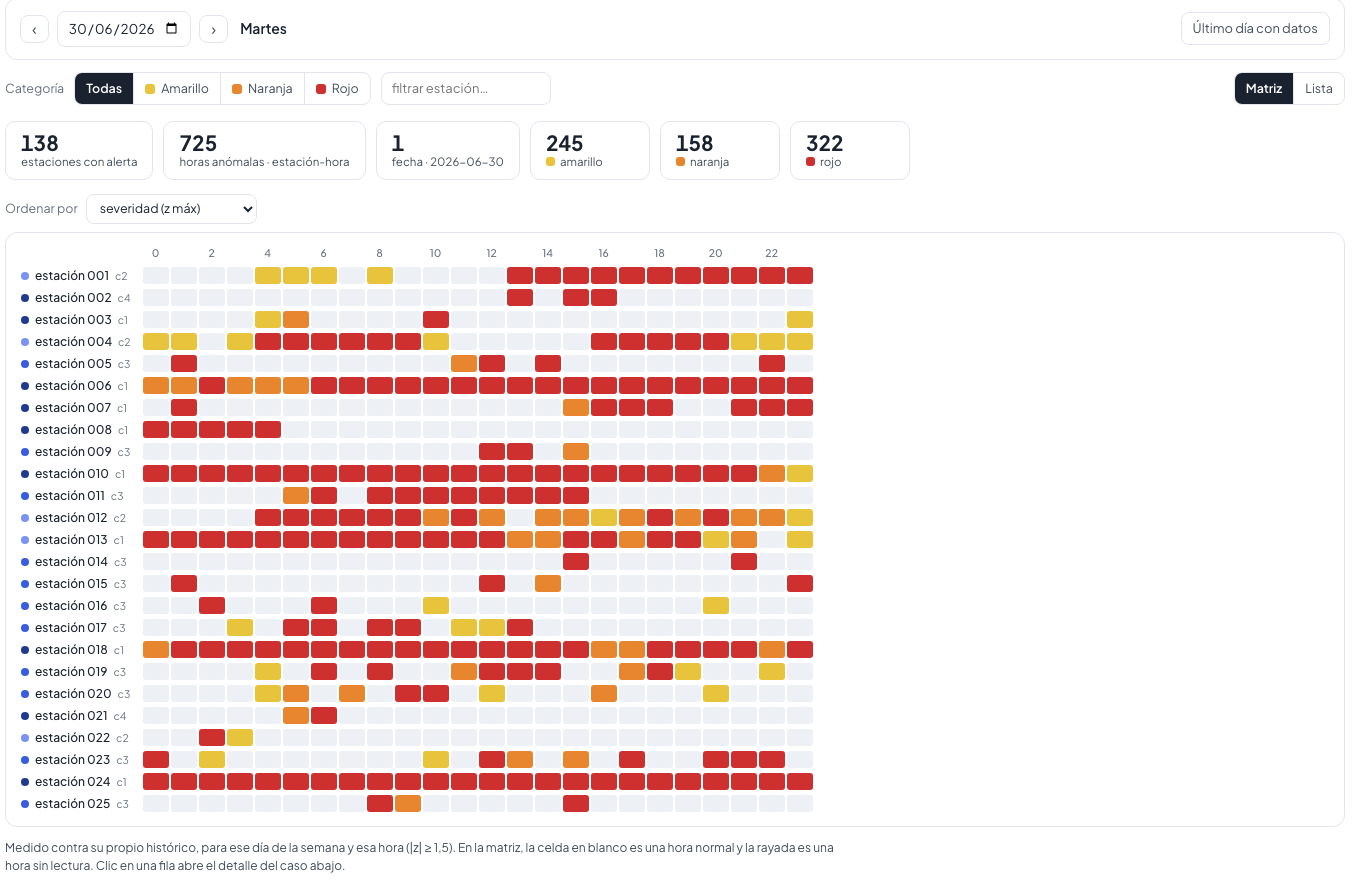
\includegraphics[height=0.62\textheight]{pic/producto_b_semaforo.png}
\end{center}

\vspace{0.15cm}
El analista elige la fecha y el sistema responde la pregunta de negocio \textbf{tal cual se formuló}: ese martes, \textbf{138 estaciones} con alerta y \textbf{725 horas--estación} anómalas, ordenadas por severidad, con la hora exacta del problema --- y un clic abre el diagnóstico del caso (volumen, temperatura, presión). \textbf{El analista de las 7:00 a.m.\ llega y la lista ya está hecha.}
\end{frame}

%%=================================================
\begin{frame}{Caso B · Del producto a la decisión}
\small
\begin{columns}[T]
\column{0.58\textwidth}
\textbf{La decisión que cambia cada día:}
\begin{itemize} \itemsep4pt
  \item \textbf{A quién revisar hoy} --- de $\sim$300 estaciones a una lista corta priorizada por severidad y por peso en el volumen.
  \item Cada caso revisado \textbf{alimenta el ciclo}: ¿era fraude, falla del medidor o un cambio real de rutina? Esa respuesta refina los umbrales del mes siguiente.
  \item Es la etapa 7 girando \textbf{cada 24 horas}: la decisión genera datos nuevos y una nueva pregunta.
\end{itemize}

\column{0.4\textwidth}
\begin{block}{\footnotesize Ficha del proyecto}
\footnotesize
\begin{itemize} \itemsep2pt
  \item Duración: \textbf{3 meses}, dos fases en paralelo.
  \item Equipo: dos científicas de datos + un consultor senior; \textbf{reunión semanal} con operaciones.
  \item Entrega: \textbf{evolutiva} (victorias tempranas $\to$ sistema).
  \item Tarea: \textbf{anomalías} (+ segmentación de apoyo).
  \item Roles protagonistas: \emph{data engineer} + \emph{data analyst}.
\end{itemize}
\end{block}
\end{columns}
\end{frame}

%%=================================================
%% SECCIÓN 4: EL CONTRASTE
%%=================================================
\section{El contraste: dos puntos de partida, dos productos}

\begin{frame}[noframenumbering]{Roadmap}
\tableofcontents[currentsection]
\end{frame}

%%=================================================
\begin{frame}{Mismo mapa, recorridos opuestos}
\footnotesize
\begin{center}
\begin{tabular}{@{}p{0.21\textwidth}p{0.35\textwidth}p{0.35\textwidth}@{}}
\toprule
 & \textbf{Caso A · Empresa P} & \textbf{Caso B · Empresa M} \\
\midrule
Necesidad & ``¿hacia dónde va nuestro mercado?'' & ``detectar consumos raros a tiempo'' \\
\rowcolor{grisclaro} Pregunta & prospectiva, horizonte 2045 & operativa, horizonte \emph{mañana} \\
Tarea analítica & predicción (supervisada) & anomalías (+ segmentación) \\
\rowcolor{grisclaro} Datos al arrancar & \textbf{no existían}: se construyó el panel desde fuentes abiertas & \textbf{sobraban}: 2,6 millones de lecturas propias \\
El esfuerzo se fue en\ldots & integrar y armonizar fuentes (etapas 2--3) & definir ``lo esperado'' y depurar (etapas 3--5) \\
\rowcolor{grisclaro} Producto & \textbf{informe} que se lee una vez & \textbf{sistema} que corre todos los días \\
Decisión & estratégica, de largo plazo & operativa, del turno de hoy \\
\rowcolor{grisclaro} Ritmo del ciclo & se revisará en años & gira cada 24 horas \\
\bottomrule
\end{tabular}
\end{center}

\vspace{0.25cm}
\begin{alertblock}{La lección}
No todos los proyectos de Business Analytics empiezan en el mismo punto ni entregan lo mismo. \textbf{La pregunta determina los datos, la tarea, el producto y el ritmo.} Por eso se formula primero.
\end{alertblock}
\end{frame}

%%=================================================
\begin{frame}{Lo que los dos casos comparten}
\small
\begin{enumerate} \setlength{\itemsep}{0.35cm}
  \item \textbf{La pregunta se escribió antes que el código.} En ambos, la parte más difícil no fue técnica: fue convertir una frase vaga en una pregunta que pasara el test.
  \item \textbf{Un baseline como vara de medir.} El promedio histórico 2020--2024 en un caso; el consumo esperado por estación en el otro. Sin punto de comparación, ningún número significa nada.
  \item \textbf{Validación honesta.} Fuera de muestra y contra el trabajo previo del cliente --- nunca contra los mismos datos que entrenaron el modelo.
  \item \textbf{El entregable habla el idioma de quien decide.} Un cuadro de prioridades gerenciales; un semáforo con la lista del día. Ninguno entrega ``el modelo''.
  \item \textbf{Ninguno empezó por el algoritmo.} El modelo apareció en la etapa 5 de 7 --- y en ambos casos fue lo \emph{menos} sofisticado del proyecto.
\end{enumerate}
\end{frame}

%%=================================================
%% SECCIÓN 5: SU TURNO
%%=================================================
\section{Su turno: el caso Cóndor}

\begin{frame}[noframenumbering]{Roadmap}
\tableofcontents[currentsection]
\end{frame}

%%=================================================
\begin{frame}{El encargo de hoy (en grupos de proyecto)}
\small
Ustedes acaban de ver dos veces el recorrido completo. Ahora arranca el suyo, con el \textbf{caso Cóndor} (el documento del caso y su diccionario de datos están en la página del curso):

\vspace{0.25cm}
\begin{enumerate} \setlength{\itemsep}{0.32cm}
  \item \textbf{Lean el caso como analistas}, no como estudiantes: ¿qué le duele a esta fintech? ¿qué decisiones está tomando a ciegas?
  \item \textbf{Inventaríen los datos}: una base principal y tres anexos. Para cada tabla que les interese: ¿qué es \emph{una fila}? ¿qué periodo cubre? ¿qué variable podría ser un \emph{target}?
  \item \textbf{Formulen UNA pregunta de negocio} que pase el test --- y clasifiquen qué tarea analítica es.
\end{enumerate}
\pause
\vspace{0.25cm}
\begin{block}{El entregable de la sesión: la ficha de su grupo}
\footnotesize
\textbf{(1)} La pregunta (específica, accionable, medible) · \textbf{(2)} la decisión que cambia con la respuesta · \textbf{(3)} las tablas/variables que la responden (incluido el target, si aplica) · \textbf{(4)} la tarea analítica y por qué.
\end{block}

\vspace{0.15cm}
Esta ficha es el \textbf{insumo directo de la Entrega 1} del proyecto final.
\end{frame}

%%=================================================
\begin{frame}{Antes de entregar: pásenle el detector}
\small
Chequeo final para su pregunta --- el mismo que usamos con las empresas P y M:

\vspace{0.25cm}
\begin{itemize} \setlength{\itemsep}{0.35cm}
  \item ¿Dice \textbf{qué, quién y cuándo}? (``mejorar la mora'' no; ``¿qué clientes de crédito entrarán en mora mayor a 30 días el próximo trimestre?'' sí.)
  \item Si les doy la respuesta ahora mismo, \textbf{¿saben qué haría Cóndor diferente mañana?} Si no hay decisión esperando, tienen un tema --- no una pregunta.
  \item ¿\textbf{Existen las columnas} para responderla en las cuatro tablas --- o al menos se pueden construir? (Recuerden la Empresa P: ``no está la columna'' a veces significa ``hay que construirla''.)
  \item ¿Qué \textbf{tarea} es? ¿Hay target histórico o no? Eso ya define la mitad de su semestre.
\end{itemize}
\pause
\vspace{0.3cm}
\begin{alertblock}{Para cerrar}
El 87\% de los proyectos de datos muere --- y casi siempre muere \textbf{en el arranque}, no en el modelo. El arranque del suyo es hoy. Háganlo como profesionales.
\end{alertblock}
\end{frame}

\end{document}
